%!TEX root = ../../super_main.tex

\section{Structuring Sensor Data}
\label{sec:modeling_sensor_data}

As stated in our vision in \secref{sec:vision}, the data collected by uMiner should be usable in various application areas, such as machine intelligence or statistics. In many of these application areas, it is beneficial if the data is structured in an uniform way. This section describes how we have tried to structure the data, and furthermore tries to concretize some of the concepts introduced in the term definition in \secref{sec:problem_definition} in relation to the developed system. 
\\\\
Conceptually, a \emph{snapshot} is a snippet of the reality (context) that a specific participant exists in, measured through the participants' devices, along with a \emph{label}, describing the context further. This label is used to define the context in ways that available sensors cannot. By examining the measured context and the labels describing these measurements, customers will be able to search for patterns in the data, and thereby might be able to see a correlation between sensor output and human dynamics. To search for temporal patterns in the data collected from the continuous- and reactive sensors, covered in \secref{sec:deriving_the_context_from_sensors}, multiple measurements are required. An example of this could be measuring the location of a participant over time to see that a user is moving. In order to see this development over time, time has to pass between every measurement. This timespan depends on what the customer desires to measure, and therefore he/she must be able to configure how long a delay there should be between every sensor reading. To define this timespan, and other aspects such as which sensors to measure from, and when to present the questionnaire to the participants, the customer must define a \emph{campaign}.
\\\\
One could imagine that a customer might be interested in finding a correlation between heart rate, movement patterns, and the influence of alcohol. In order to do this, a customer could create a campaign, in which he specifies which information should be gathered from the sensors, such as heart rate, acceleration, and GPS location. The customer would furthermore specify questions for the participants, asking whether they are, or have been, under the influence of alcohol at a specific time. One could alternatively utilize a breathalyzer, but these are not common in mobile devices, making a questionnaire a viable alternate method for distinguishing if the participant has consumed alcohol. The created specification can then be used as a recipe for creating and submitting snapshots, possibly including labels provided by participants. An illustration of how a snapshot is structured can be seen in \figref{fig:snapshot_model_no_samples}, which shows how time elapses between every measurement. In this example, the participants are asked to answer the question: \emph{Are you under the influence of alcohol?} in order to label the data.
\\
\begin{figure}[!htbp]
    \centering
    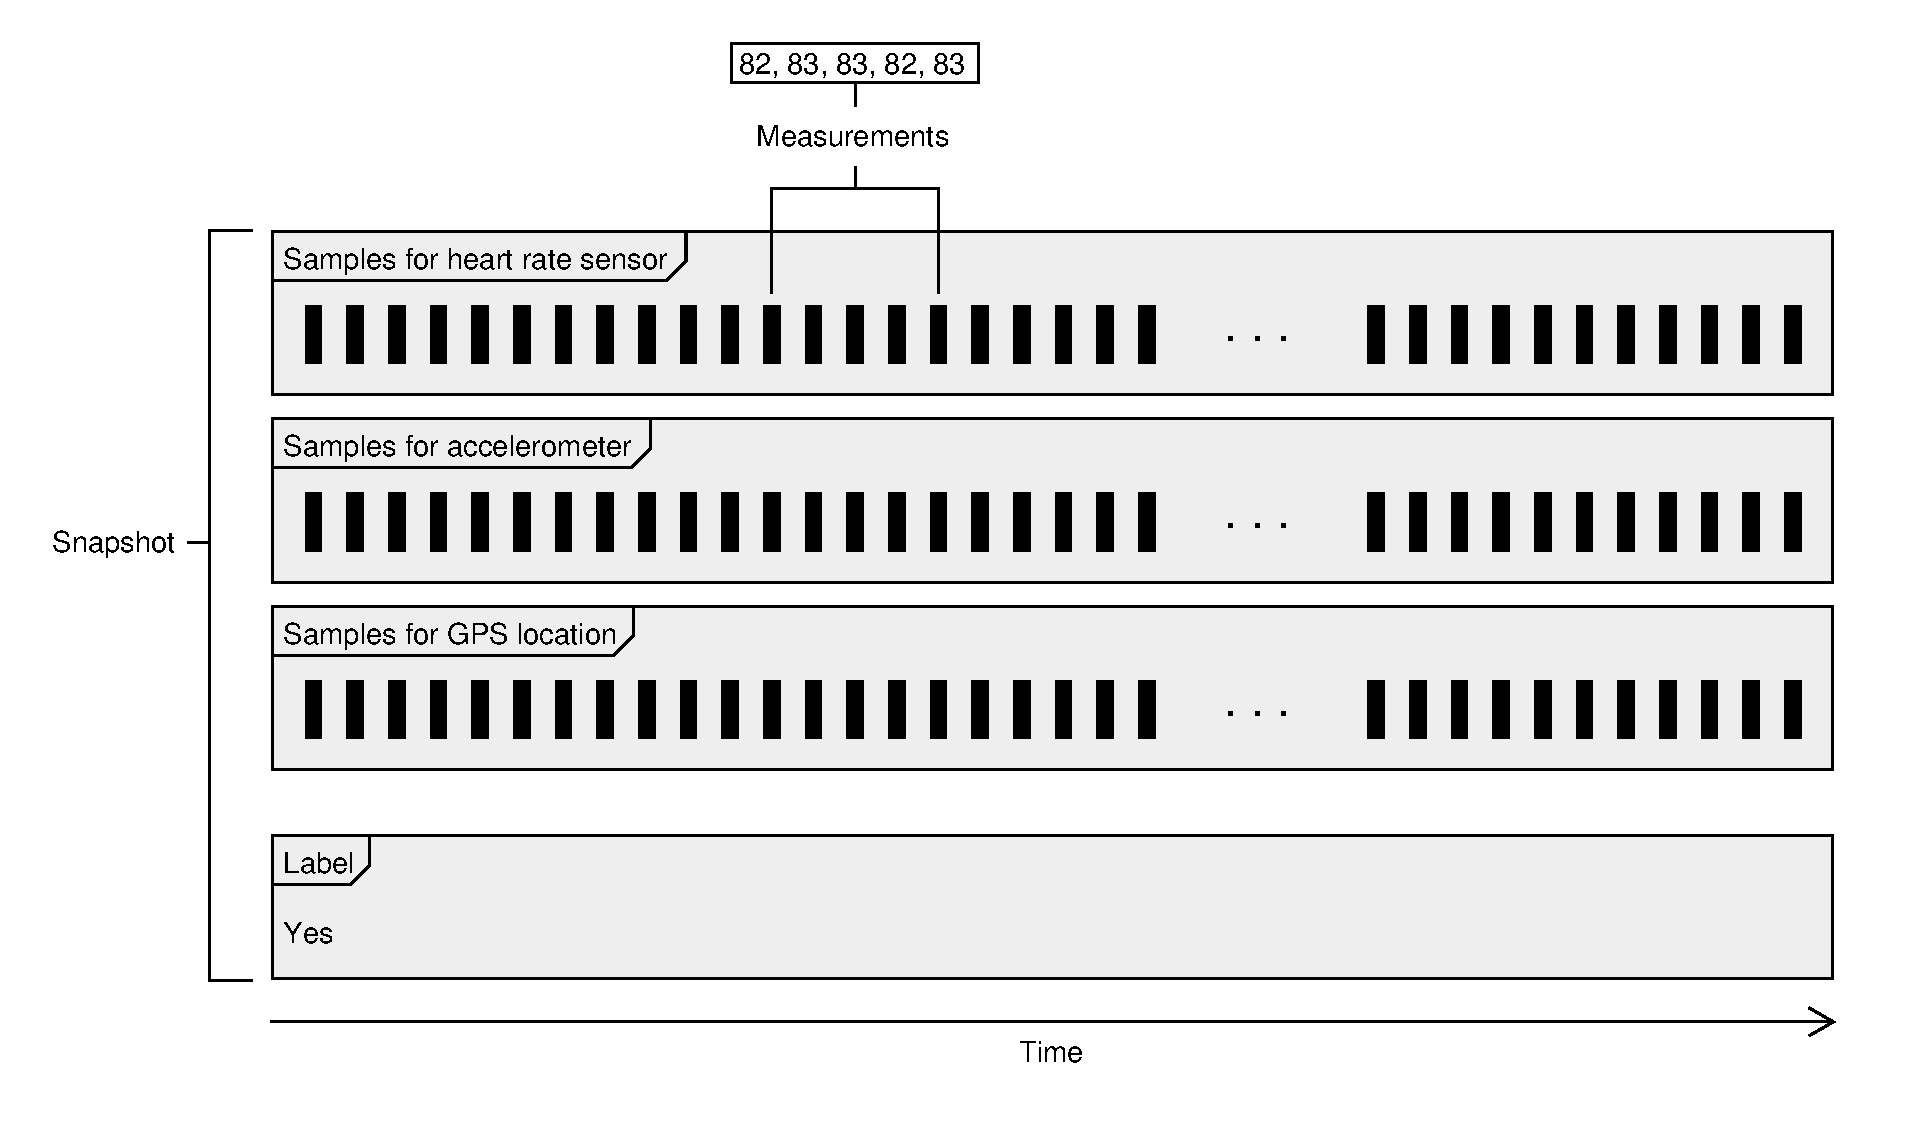
\includegraphics[width=\textwidth]{gathering_sensor_data/snapshot_model_no_samples}
    \caption{Snapshot example containing measurements from three sensors and a label.}
    \label{fig:snapshot_model_no_samples}
\end{figure}
\FloatBarrier

%!TEX root = ../../super_main.tex

\subsection{Data Quantity Estimation}
\label{sec:data_quantity_estimation}
%This gave us a dataset with a size of 142908 bytes. This experiment would then yield a data set of approximately 205 MB if it was run for a day. Running the same experiment for 30 days with 100 different devices would then approximately yield a data set of 617 GB assuming similar mobile devices with similar sensors. This quick napkin math was only for one sensor with 100 people and this could quickly escalate if more sensor or more people are added.

\todo[inline]{Overvej: Lav en reference til vores user story, og fortæl hvor meget data vi samler om dagen med disse målinger. Skriv også at dette KUN er RÅ sensor output, stored i Java-hukommelse størrelser. Med snapshot struktur er det meget værre} 

According to our problem statement in \secref{sub:problem_statement}, we want to minimize the effect that our application has on the  daily mobile lives of participants. One aspect that might have influence on this is the battery consumption and network usage of our application. We would there like to minimize these factors. In order to do this, we have experimented with different continuous sensors on a Nexus 5 smartphone and logged all values captured from the sensor for 1, 5, and 20 minutes. The results of these tests can be seen in \tabref{tab:sensor_experiment}. Note that the orientation sensor is a virtual sensor, which uses data collected from both the gyroscope and magnetometer, hence the correlation between the data sizes ($143 \text{KB} + 35 \text{KB} \approx 177 \text{KB}$ for 1 minute). These tests were only performed for four different sensors, but customers might need data from several different sensors, thus further increasing the amount of data collected. These quantities of data might present a problem even on modern mobile platforms due to paid limited data plans and battery consumption. There might be different data needs, some customers might require very detailed data from many sensors from a few devices and others might require more sparse data from a few sensors from a lot of different devices. However, we can conclude that gathering a continuous stream of data from all sensors all the time is not a viable solution.

\begin{table}[!htbp]
\centering
\begin{tabular}{l|c|c|c|c}
\textbf{Sensor}     & \textbf{Accellerometer} & \textbf{Gyroscope} & \textbf{Magnetometer} & \textbf{Orientation} \\ \hline
\textbf{1 minute}   & 142 KB                  & 143 KB             & 35 KB                 & 177 KB               \\ \hline
\textbf{5 minutes}  & 714 KB                  & 714 KB             & 178 KB                & 892 KB               \\ \hline
\textbf{20 minutes} & 2,859 KB                & 2,859 KB           & 715 KB                & 3,573 KB                
\end{tabular}
\caption{Data size of sensor data collection after a set amount of time.}
\label{tab:sensor_experiment}
\end{table}
\FloatBarrier

\subsection{Temporal Properties of Snapshots}
\label{sec:temporal_properties_of_snapshots}

\todo[inline]{META: De følgende to todos er forsøgt løst, men ved ikke hvor godt det er. Den gamle tekst står udkommenteret i dokumentet. Er lidt i tvivl om vi kan bruge data estimation til noget her da testen er kørt event driven... Todo nummer tre har jeg ikke kunne få skrevet ind...}
\todo[inline]{Skriv en opdateret introduktion der er baseret på \secref{sec:data_quantity_estimation}, der forklarer hvorfor vi har behov for samples, og deres delay. Det er IKKE fordi kunderne synes at det er godt!}

As previously mentioned, we would need more than a single reading from a sensor in order to search for temporal patterns in the data, which is why we introduce the \emph{measurement} concept shown in \figref{fig:snapshot_model_no_samples}. However, using a raw data stream from the sensors resulted in large quantities of data as covered in the previous section. This data would have to be sent over the Internet to enable us to show it to the customers. This is, as mentioned in \secref{sec:general_strategies}, a task that might consume a lot of power. 

\todo[inline]{Beskriv konflikten mellem customers og participants (kunder vil gerne have meget data, men participants kun vil give så lidt som muligt).}

This presents a conflict between the customers and the participants of the system. The customers would probably like to receive as much data as possible, whereas the participants would like the collection to affect their phone as little as possible. One could argue that the customers would be interested in lowering the power consumption and bandwidth usage on the participants devices because they would like to avoid discouraging them from contributing to their campaign. 
\\\\
In order to solve this conflict we have introduced a span between a sequence of \emph{measurements}, that the customer can regulate in order to reduce the battery and network consumption on the participants' devices. To be able to talk about this sequence of measurements we introduce another concept that we call \emph{sample}. A \emph{sample} is simply such a sequence of \emph{measurements} with an interval between them, as seen in \figref{fig:snapshot_example_with_samples}. This allows customers to make sense of continuous sensor readings, but in a periodic manner, that avoids unnecessary strain on the participants' devices.



\todo[inline]{Beskriv at det er et krav at mellemrummet mellem measurements er konstant, så vi kan sammenligne measurement på index x i et sample for sensor 1, sammen med index x i et andet sample for sensor 2. Alternativt kunne man tage et timestamp på alle measurements, men det vil tage meget plads at sende, så istedet vil vi gerne have et timestamp på sample, og en relativ tid på measurements.}

% A single sensor reading from a continuous sensor often does not make much sense on its own, which is why we introduced the \emph{measurement} concept. Following the introduction of measurements, we came to the realization that customers might be interested in taking a stream of measurements, waiting for some amount of time, and then taking another stream of measurements. The customers might need data sequences that is separated by some span larger than the one between measurements. However, the more apparent benefit of this is to encourage the participants to join, due to reduced strain on their hardware. In introducing a span between a sequence of measurements the customer can regulate this in order to reduce the amount of data send to the server, which will reduce the battery and network consumption on the participants' devices. This has led to the introduction of a concept that we call \emph{sample}. A \emph{sample} is simply a sequence of \emph{measurement}s with an interval between them, as seen in \figref{fig:snapshot_example_with_samples}. This allows customers to make sense of continuous sensor readings, but in a periodic manner, that avoids unnecessary strain on the participants' devices.

\begin{figure}[!htbp]
    \centering
    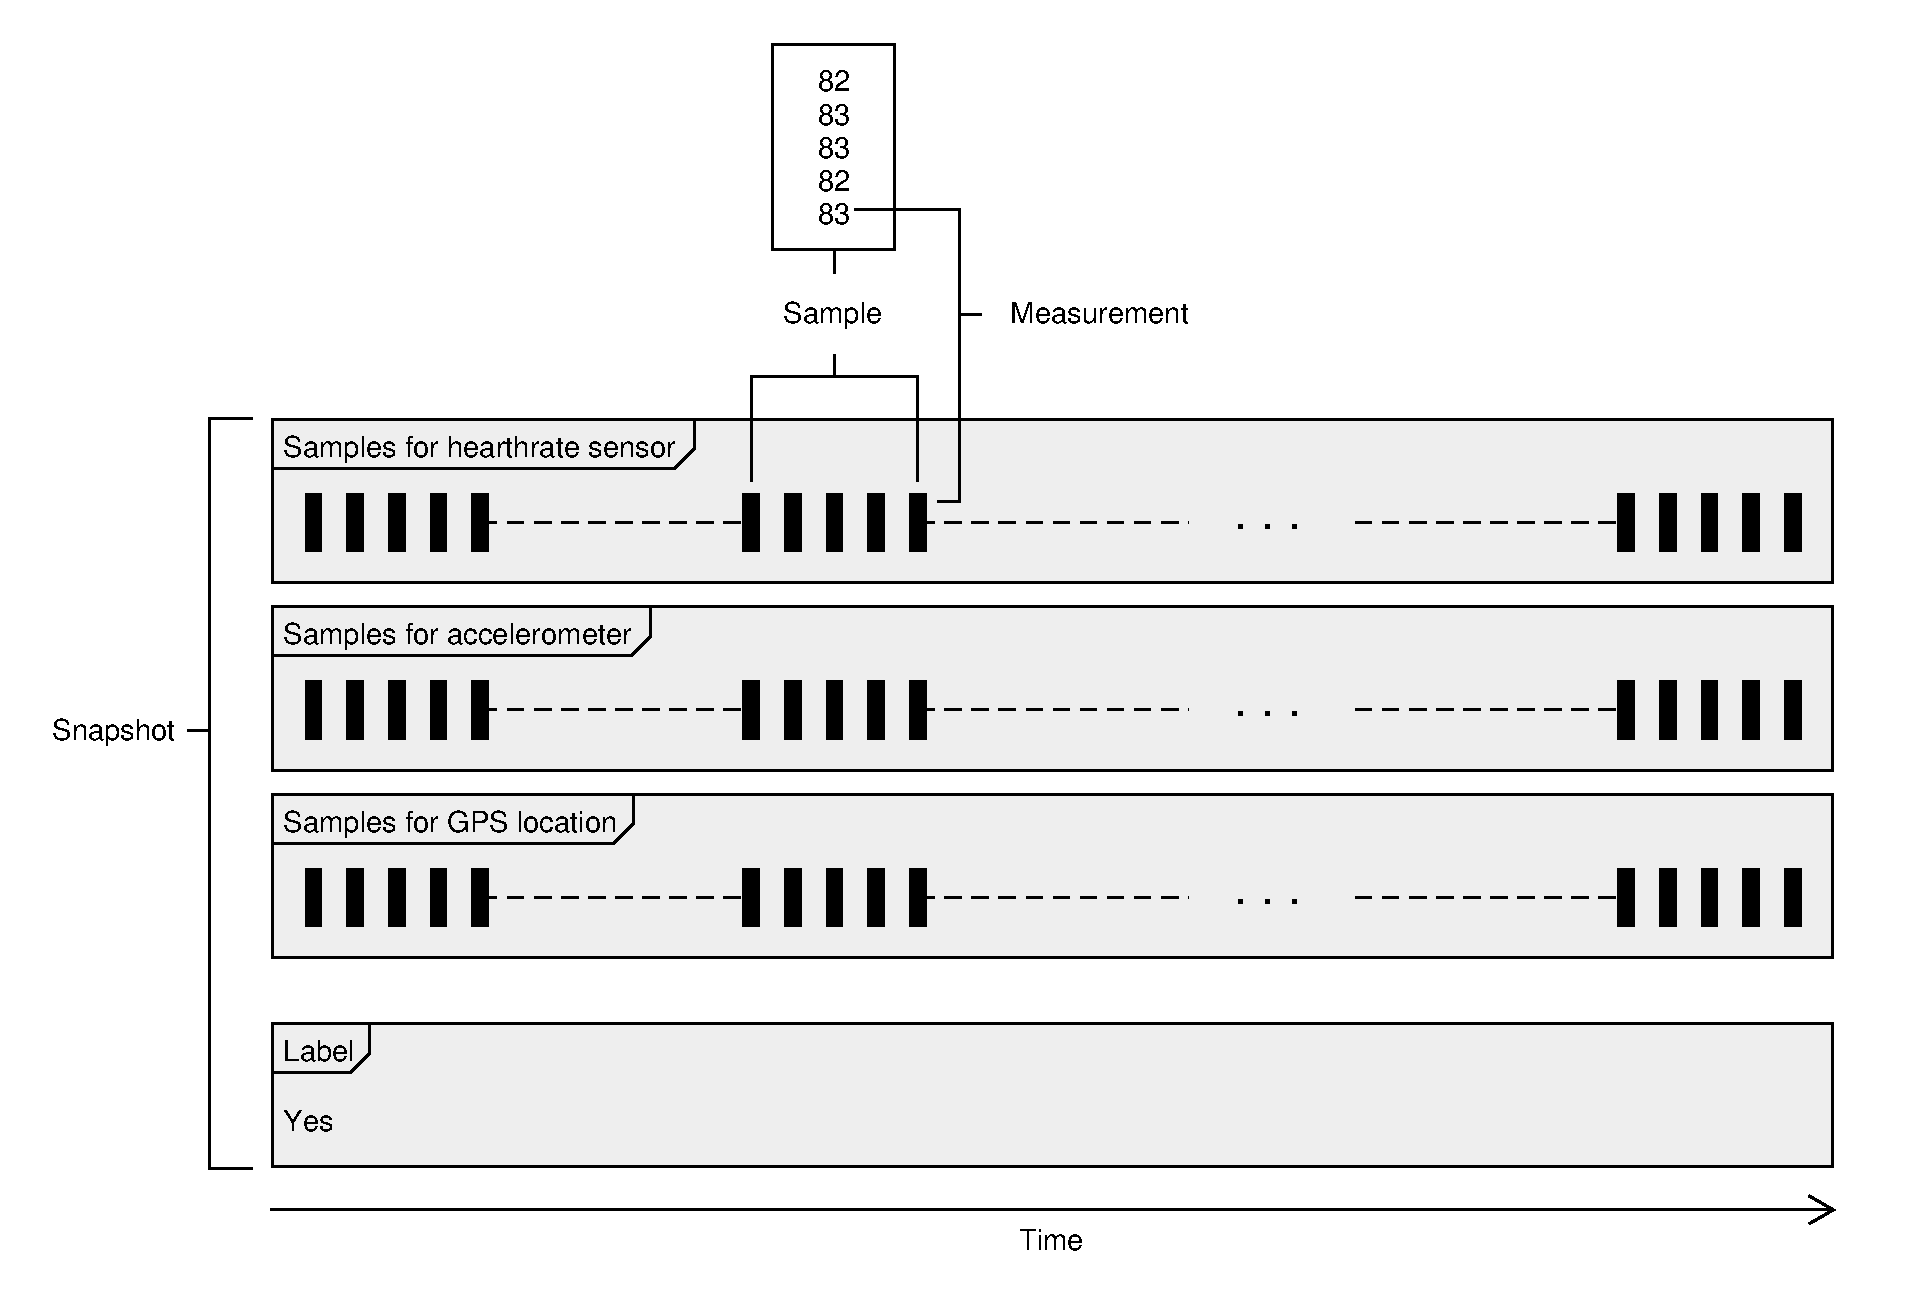
\includegraphics[width=\textwidth]{gathering_sensor_data/snapshot}
    \caption{Snapshot example containing samples from three sensors and a label.}
    \label{fig:snapshot_example_with_samples}
\end{figure}
\FloatBarrier

We want customers to configure how often \emph{measurement}s should be made, and we therefore allow them to define a \emph{measurement frequency} for their \emph{campaign}. Customers should furthermore be able to define how often \emph{sample}s should be gathered, and for that reason we allow them to define a \emph{sample frequency}. Lastly, the length of the \emph{snapshot} is configurable by defining how many \emph{sample}s the customer wants for a single \emph{snapshot}. This is used to calculate what we call \emph{total duration}, which states for how long samples should be generated for a snapshot. All of this is illustrated in \figref{fig:sample_temporality}. 

\todo[inline]{Skriv hvordan label'en kommer ind i billedet. Det skal forklares i dybden, og ikke bare være en sidenote
. Før stod der: Lastly, a customer should be able to define when the questionnaire should appear to the participant, for example at the start or the end of a snapshot.}

\begin{figure}[!htbp]
    \centering
    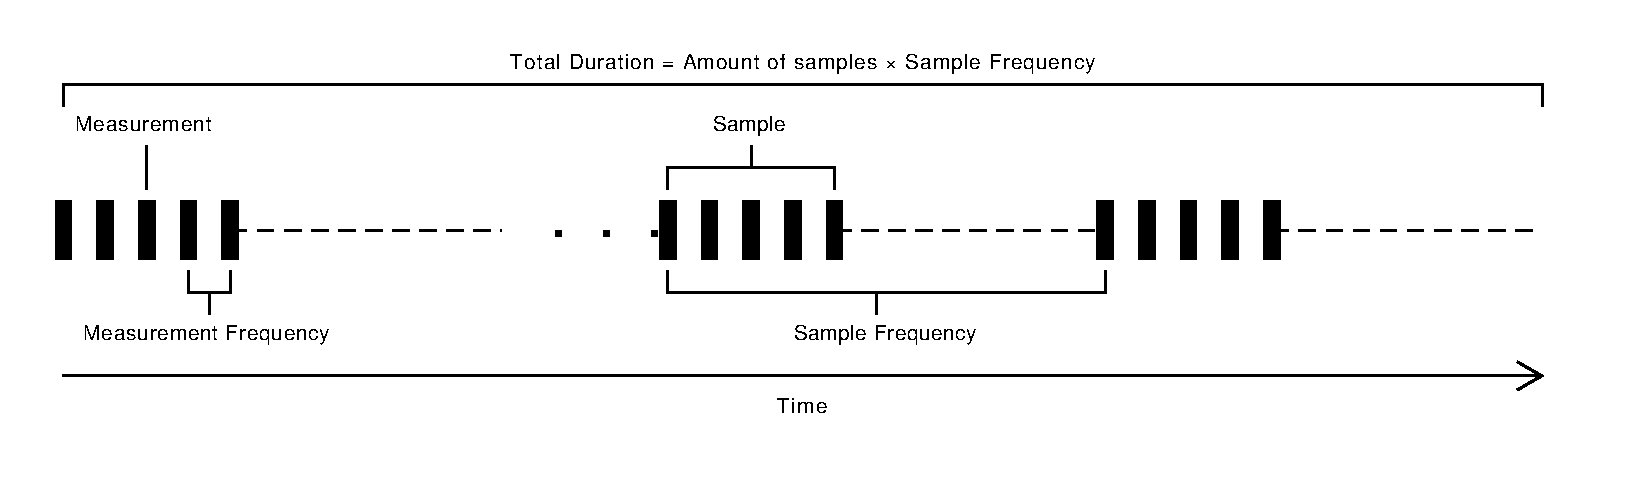
\includegraphics[width=\textwidth]{gathering_sensor_data/sample_temporality}
    \caption{Illustration of temporality for samples for a single sensor in a snapshot.}
    \label{fig:sample_temporality}
\end{figure}
\FloatBarrier

By this temporal structure of the sensor data we provide a viable way of configuring how the snapshots should be structured in regards to sensor readings, while maintaining a uniform output format for customers of the system.
